\documentclass{article}%
\usepackage[T1]{fontenc}%
\usepackage[utf8]{inputenc}%
\usepackage{lmodern}%
\usepackage{textcomp}%
\usepackage{lastpage}%
\usepackage[head=40pt,margin=0.5in,bottom=0.6in]{geometry}%
\usepackage{graphicx}%
%
\title{\textbf{Qué implica que seis países hayan pedido a la CPI investigar a Maduro}}%
\author{NO\_TIENE}%
\date{27/09/2018}%
%
\begin{document}%
\normalsize%
\maketitle%
\textbf{URL: }%
http://www.el{-}nacional.com/noticias/bbc{-}mundo/que{-}implica{-}que{-}seis{-}paises{-}hayan{-}pedido{-}cpi{-}investigar{-}maduro\_253402\newline%
%
\textbf{Periodico: }%
EN, %
ID: %
253402, %
Seccion: %
BBC Mundo\newline%
%
\textbf{Palabras Claves: }%
Nicolás Maduro, Luis Almagro, Gobierno\newline%
%
\textbf{Derecho: }%
18, %
Otros Derechos: %
5, %
Sub Derechos: %
\newline%
%
\textbf{EP: }%
NO\newline%
\newline%
%
\textbf{\textit{La denuncia realizada por cinco países latinoamericanos y Canadá en contra del gobierno nacional crea una situación inédita en el tribunal creado para juzgar los crímenes de lesa humanidad}}%
\newline%
\newline%
%
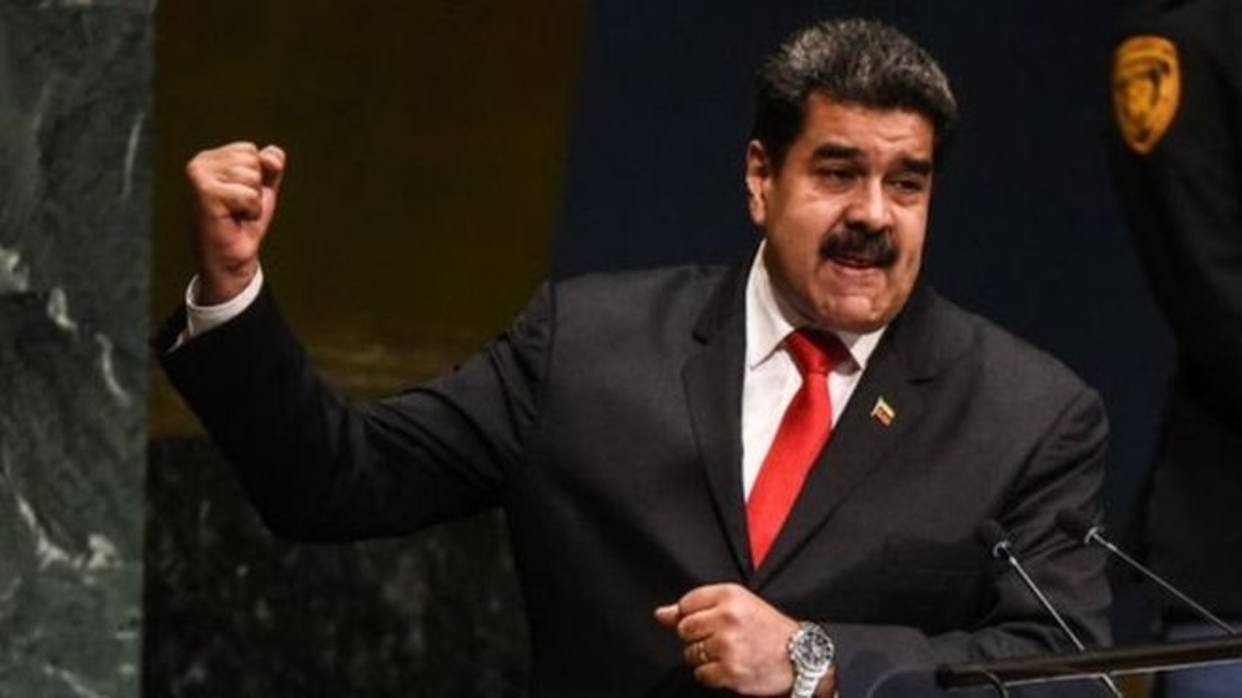
\includegraphics[width=300px]{224.jpg}%
\newline%
%
Se trata de una situación completamente inédita.%
\newline%
%
Este miércoles los gobiernos de Argentina, Chile, Colombia, Paraguay, Perú y Canadá solicitaron a la fiscalía de la Corte Penal Internacional (CPI) que investigue supuestos crímenes de lesa humanidad y abusos a los derechos humanos ocurridos en Venezuela desde el 12 de abril de 2014 bajo el gobierno de Nicolás Maduro.%
\newline%
%
Nunca antes desde la entrada en funciones de ese tribunal con sede en La Haya (Holanda) en 2002, se había dado el caso de que Estados parte del Estatuto de Roma, la norma internacional que creó la CPI, pidieran abrir un procedimiento contra otro estado miembro.%
\newline%
%
"Lo novedoso de este proceso es que quienes hacen la denuncia son jefes de~Estado y de gobierno, porque los casos anteriores obedecieron al trabajo de documentación de organizaciones de derechos humanos que los llevaron ante la Fiscalía de la CPI", explica Juan Navarrete, exrepresentante en Colombia del Instituto Interamericano de Derechos Humanos, en conversación con BBC Mundo.%
\newline%
%
El experto destaca que, a diferencia de los casos que se procesan a través de otros organismos como, por ejemplo, la Corte Interamericana de Derechos Humanos, en los juicios que se procesan ante la CPI la responsabilidad no es del Estado sino individual.%
\newline%
%
"Aunque se habla de la denuncia contra Venezuela,~no se va contra el~Estado venezolano sino contra las personas señaladas por violaciones de derechos humanos y delitos de lesa humanidad. Además, aunque ellos mencionen a Maduro, siempre en la investigación se afecta a toda la cadena de mando que hizo posibles esos hechos", agrega.%
\newline%
%
El secretario general de la OEA, Luis Almagro, ha sido uno de los principales críticos del gobierno de Maduro%
\newline%
%
Navarrete destaca que esta denuncia también pudo haber sido hecha a través del Consejo de Seguridad de la ONU pero, en ese caso, tenía que contar con la aprobación de la mayoría de sus miembros y sortear el derecho a veto de los miembros permanentes (Estados Unidos, Rusia, China, Reino Unido y Francia).%
\newline%
%
La solicitud de investigación contra Venezuela se fundamenta, entre otros elementos, en tres informes sobre violaciones a los derechos humanos en ese país elaborados por la ONU, la Organización de Estados Americanos (OEA) y por la Comisión Interamericana de Derechos Humanos (CIDH).%
\newline%
%
En la noche de este miércoles, en su discurso ante la ONU pocas horas más tarde de la presentación de la denuncia, Maduro dijo que existe~una conspiración internacional~en contra de su gobierno.%
\newline%
%
¿Y ahora qué pasará?%
\newline%
%
La fiscal de la CPI, Fatou Bensouda, deberá decidir qué hacer con la denuncia contra Venezuela%
\newline%
%
La Fiscalía de la CPI abrió de oficio en febrero de este año una investigación preliminar para determinar si en Venezuela, al menos desde abril de 2017, se habían cometido crímenes que fueran de competencia de ese tribunal.%
\newline%
%
Según explica Fernando Fernández, profesor de Derecho Penal Internacional en la Universidad Central de Venezuela, ese tipo de procedimientos pueden durar años, como ha ocurrido con un proceso sobre el conflicto interno de Colombia que se encuentra en esa etapa desde 2004.%
\newline%
%
Cuando se encuentran elementos suficientes sobre un caso, usualmente los resultados de esas primeras indagaciones son llevados por la Fiscalía ante la Sala de Cuestiones Preliminares (SCP), una suerte de tribunal de control que~decide si se cumplen las condiciones para admitir la causa y dar luz verde a una investigación final con miras a realizar un juicio penal.%
\newline%
%
El experto indica que con la petición de una investigación presentada este miércoles, lo que ocurra con el caso venezolano puede ser distinto.%
\newline%
%
"Ahora la Fiscalía está en situación de actuar. Esa es la importancia de este paso. Tiene que determinar si abre una investigación final por su cuenta o si lleva primero el caso ante la SCP. Hay una interpretación jurídica que dice que en este caso no necesitaría ir a la SCP porque existe la petición de los Estados, pero esa~es una cuestión que se va a dilucidar ahora porque es primera vez que ocurre", señala.%
\newline%
%
La CPI abrió una investigación preliminar para determinar si en Venezuela se cometieron crímenes de lesa humanidad%
\newline%
%
Si la Fiscalía acude a la SCP y esta admite la causa se iniciaría la investigación formal con todos los elementos usuales: recolección de pruebas, citación de testigos, realización de cuestionarios a los acusados, exhumación de cadáveres, etc.%
\newline%
%
Una vez concluida la investigación, sus resultados serían presentados ante la SCP para que esta autorice la realización del juicio.%
\newline%
%
Si en cualquiera de estas etapas, durante la investigación preliminar o la final, la SCP rechaza el caso entonces habría que esperar al surgimiento de nuevos elementos para poder volver a presentarlo.%
\newline%
%
Precedentes%
\newline%
%
Fernández destaca que todo~lo que ocurra a partir de ahora con la~solicitud de investigación~contra Venezuela será muy importante porque sentará un precedente.%
\newline%
%
"Esto pone a prueba el Estatuto de Roma en toda su capacidad porque mide su fortaleza como institución procesal", señala.%
\newline%
%
El experto señala que este procedimiento puede ser rápido si las partes colaboran, pero que si no lo hacen como ocurrió el en caso del presidente de Sudán, Omar al{-}Bashir, las cosas se pueden estancar.%
\newline%
%
En 2008, la Fiscalía de la CPI acusó al mandatario sudanés de cargos de genocidio por crímenes de guerra cometidos en la región de Darfur.%
\newline%
%
Sobre el presidente de Sudán, Omar al{-}Bashir, pesa una orden internacional de detención emitida por la CPI%
\newline%
%
Al{-}Bashir se convirtió así en el primer Jefe de Estado en funciones en ser imputado por esa instancia.%
\newline%
%
El gobierno sudanés rechazó las acusaciones y no ha querido colaborar con el proceso, por lo cual Al{-}Bashir no ha podido ser juzgado aún.%
\newline%
%
Eso, sin embargo, no le ha evitado pasar algunos malos ratos.~La CPI emitió en 2009 y 2010 dos órdenes de captura en su contra, lo que le ha dificultado realizar viajes al extranjero.%
\newline%
%
En 2015, por ejemplo, Al{-}Bashir tuvo que abandonar apresuradamente Sudáfrica, donde asistía a una cumbre de la Unión Africana, para evadir la orden de un juez local que acordó su arresto para cumplir con la decisión de la CPI.%
\newline%
%
Los jueces de ese tribunal han dicho que todos los países firmantes del Estatuto de Roma están en la obligación de detenerle.%
\newline%
%
Hasta ahora, el mandatario sudanés ha evitado su captura y ha seguido viajando, principalmente a lugares de África y Asia.%
\newline%
%
Sin embargo, no ha pisado Estados Unidos, Europa occidental ni otros países en los que podría ser detenido.%
\newline%
%
El mundo, al parecer, se le ha hecho un poco más pequeño.%
\newline%
%
\end{document}